\documentclass{article}
\usepackage[left=0.5in,top=0.5in,right=0.5in,bottom=0.5in]{geometry}
\usepackage[english]{babel}
\usepackage[utf8]{inputenc}
\usepackage[table]{xcolor}
\usepackage{amssymb,amsmath,amsthm}
\usepackage{changepage,threeparttable}
\usepackage{booktabs,multirow}
\usepackage{graphicx}
\usepackage{soul}
\graphicspath{{./images/}}
\def\F#1{\(#1\)}
\title{Lab 8: The RC Filter}
\author{Philip Kim}
\date{\today}
\begin{document}
\maketitle
\vspace*{-1cm}

\begin{table}[!htp]\centering
  \begin{tabular}{|c|c|c|c|c|c|c|c|c|}\hline
    \multicolumn{9}{|c|}{\textbf{Table 1: High-Pass Filter}} \\\hline
    \F{f_{gen}}&\F{f_{osc}}&\F{C}&\F{R}&\F{V_{RC}}&\F{V_{R}}&\F{V/DIV~for~V_R}&\F{\left|H_{exp}\right|}&\F{\left|H_{the}\right|}\\\hline
    10kHz& &0.22\(\mu{F}\)&100\F{\Omega}& & & & & \\\hline
    5kHz& &0.22\(\mu{F}\)&100\F{\Omega}& & & & & \\\hline
    2kHz& &0.22\(\mu{F}\)&100\F{\Omega}& & & & & \\\hline
    1kHz& &0.22\(\mu{F}\)&100\F{\Omega}& & & & & \\\hline
    15kHz& &0.22\(\mu{F}\)&100\F{\Omega}& & & & & \\\hline
    20kHz& &0.22\(\mu{F}\)&100\F{\Omega}& & & & & \\\hline
    30kHz& &0.22\(\mu{F}\)&100\F{\Omega}& & & & & \\\hline
    40kHz& &0.22\(\mu{F}\)&100\F{\Omega}& & & & & \\\hline
  \end{tabular}
\end{table}

\begin{table}[!htp]\centering
  \begin{tabular}{|c|c|c|c|c|c|c|c|c|}\hline
    \multicolumn{9}{|c|}{\textbf{Table 2: Low-Pass Filter}} \\\hline
    \F{f_{gen}}&\F{f_{osc}}&\F{C}&\F{R}&\F{V_{RC}}&\F{V_{C}}&\F{V/DIV~for~V_C}&\F{\left|H_{exp}\right|}&\F{\left|H_{the}\right|}\\\hline
    10kHz& &0.22\(\mu{F}\)&100\F{\Omega}& & & & & \\\hline
    5kHz& &0.22\(\mu{F}\)&100\F{\Omega}& & & & & \\\hline
    2kHz& &0.22\(\mu{F}\)&100\F{\Omega}& & & & & \\\hline
    1kHz& &0.22\(\mu{F}\)&100\F{\Omega}& & & & & \\\hline
    15kHz& &0.22\(\mu{F}\)&100\F{\Omega}& & & & & \\\hline
    20kHz& &0.22\(\mu{F}\)&100\F{\Omega}& & & & & \\\hline
    30kHz& &0.22\(\mu{F}\)&100\F{\Omega}& & & & & \\\hline
    40kHz& &0.22\(\mu{F}\)&100\F{\Omega}& & & & & \\\hline
  \end{tabular}
\end{table}

\begin{center}
  \subsection*{Setup}
  % 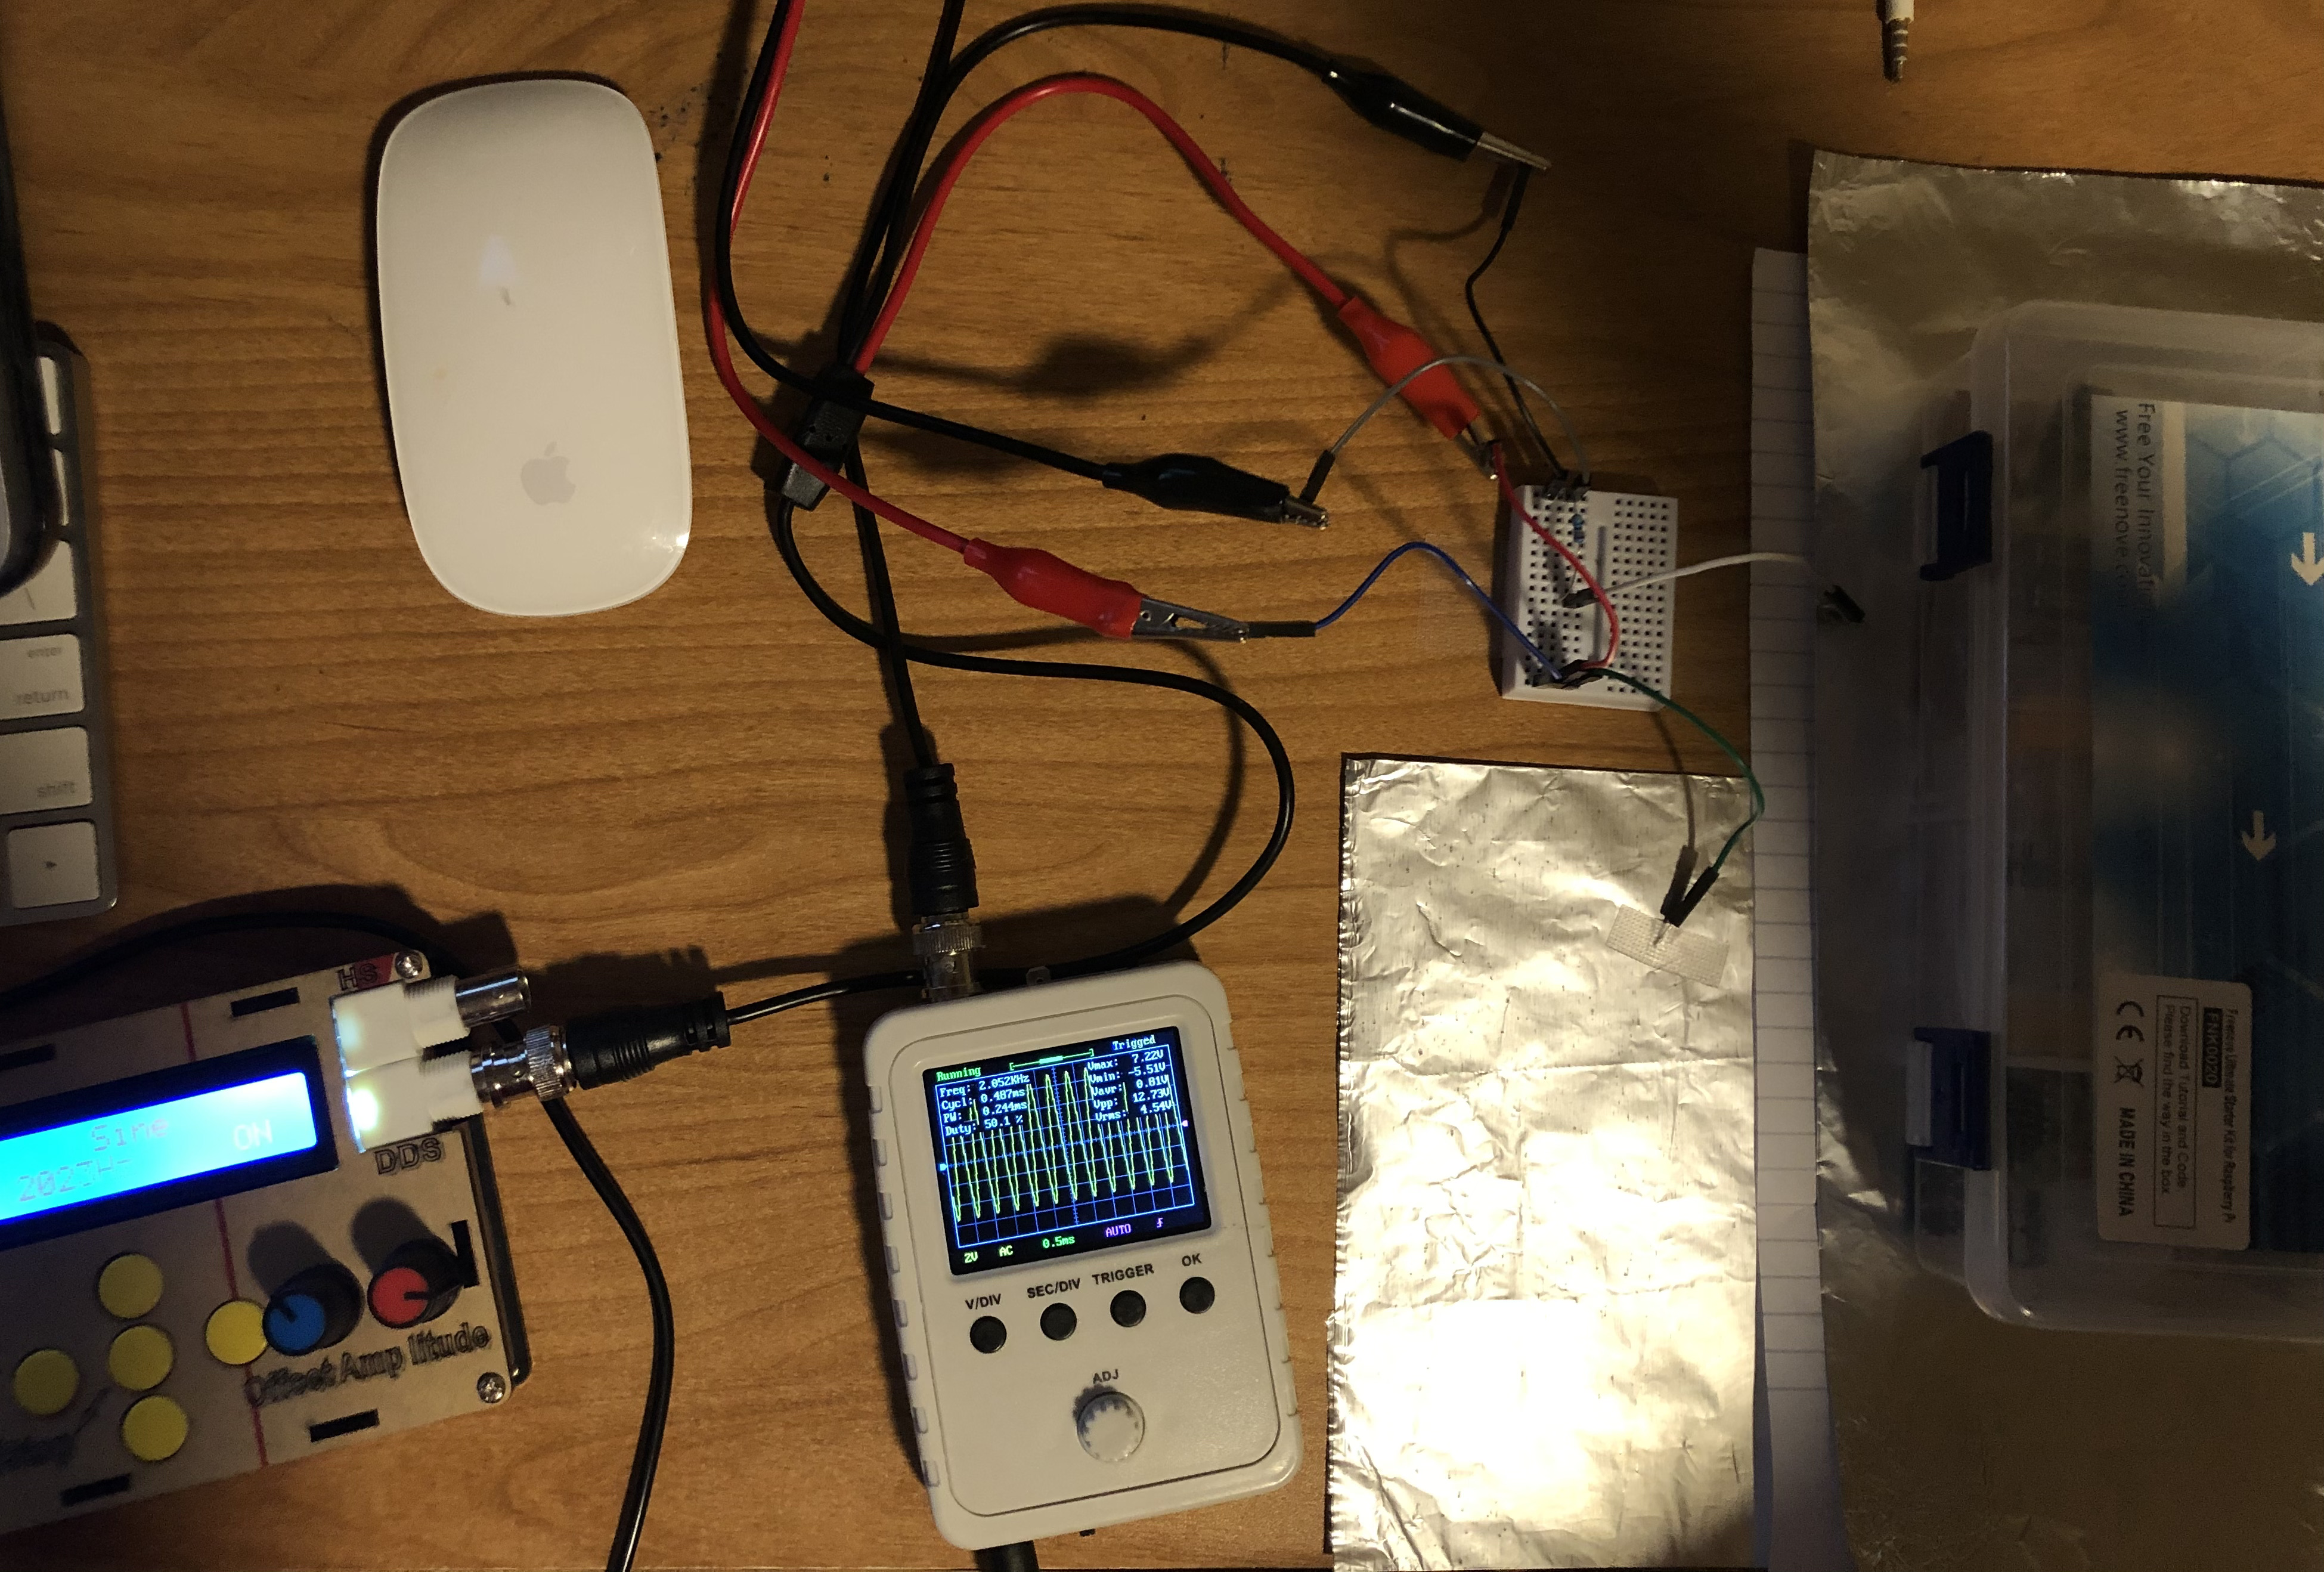
\includegraphics[scale=0.07]{VRC.jpeg}
  % \subsection*{Setup}
  % 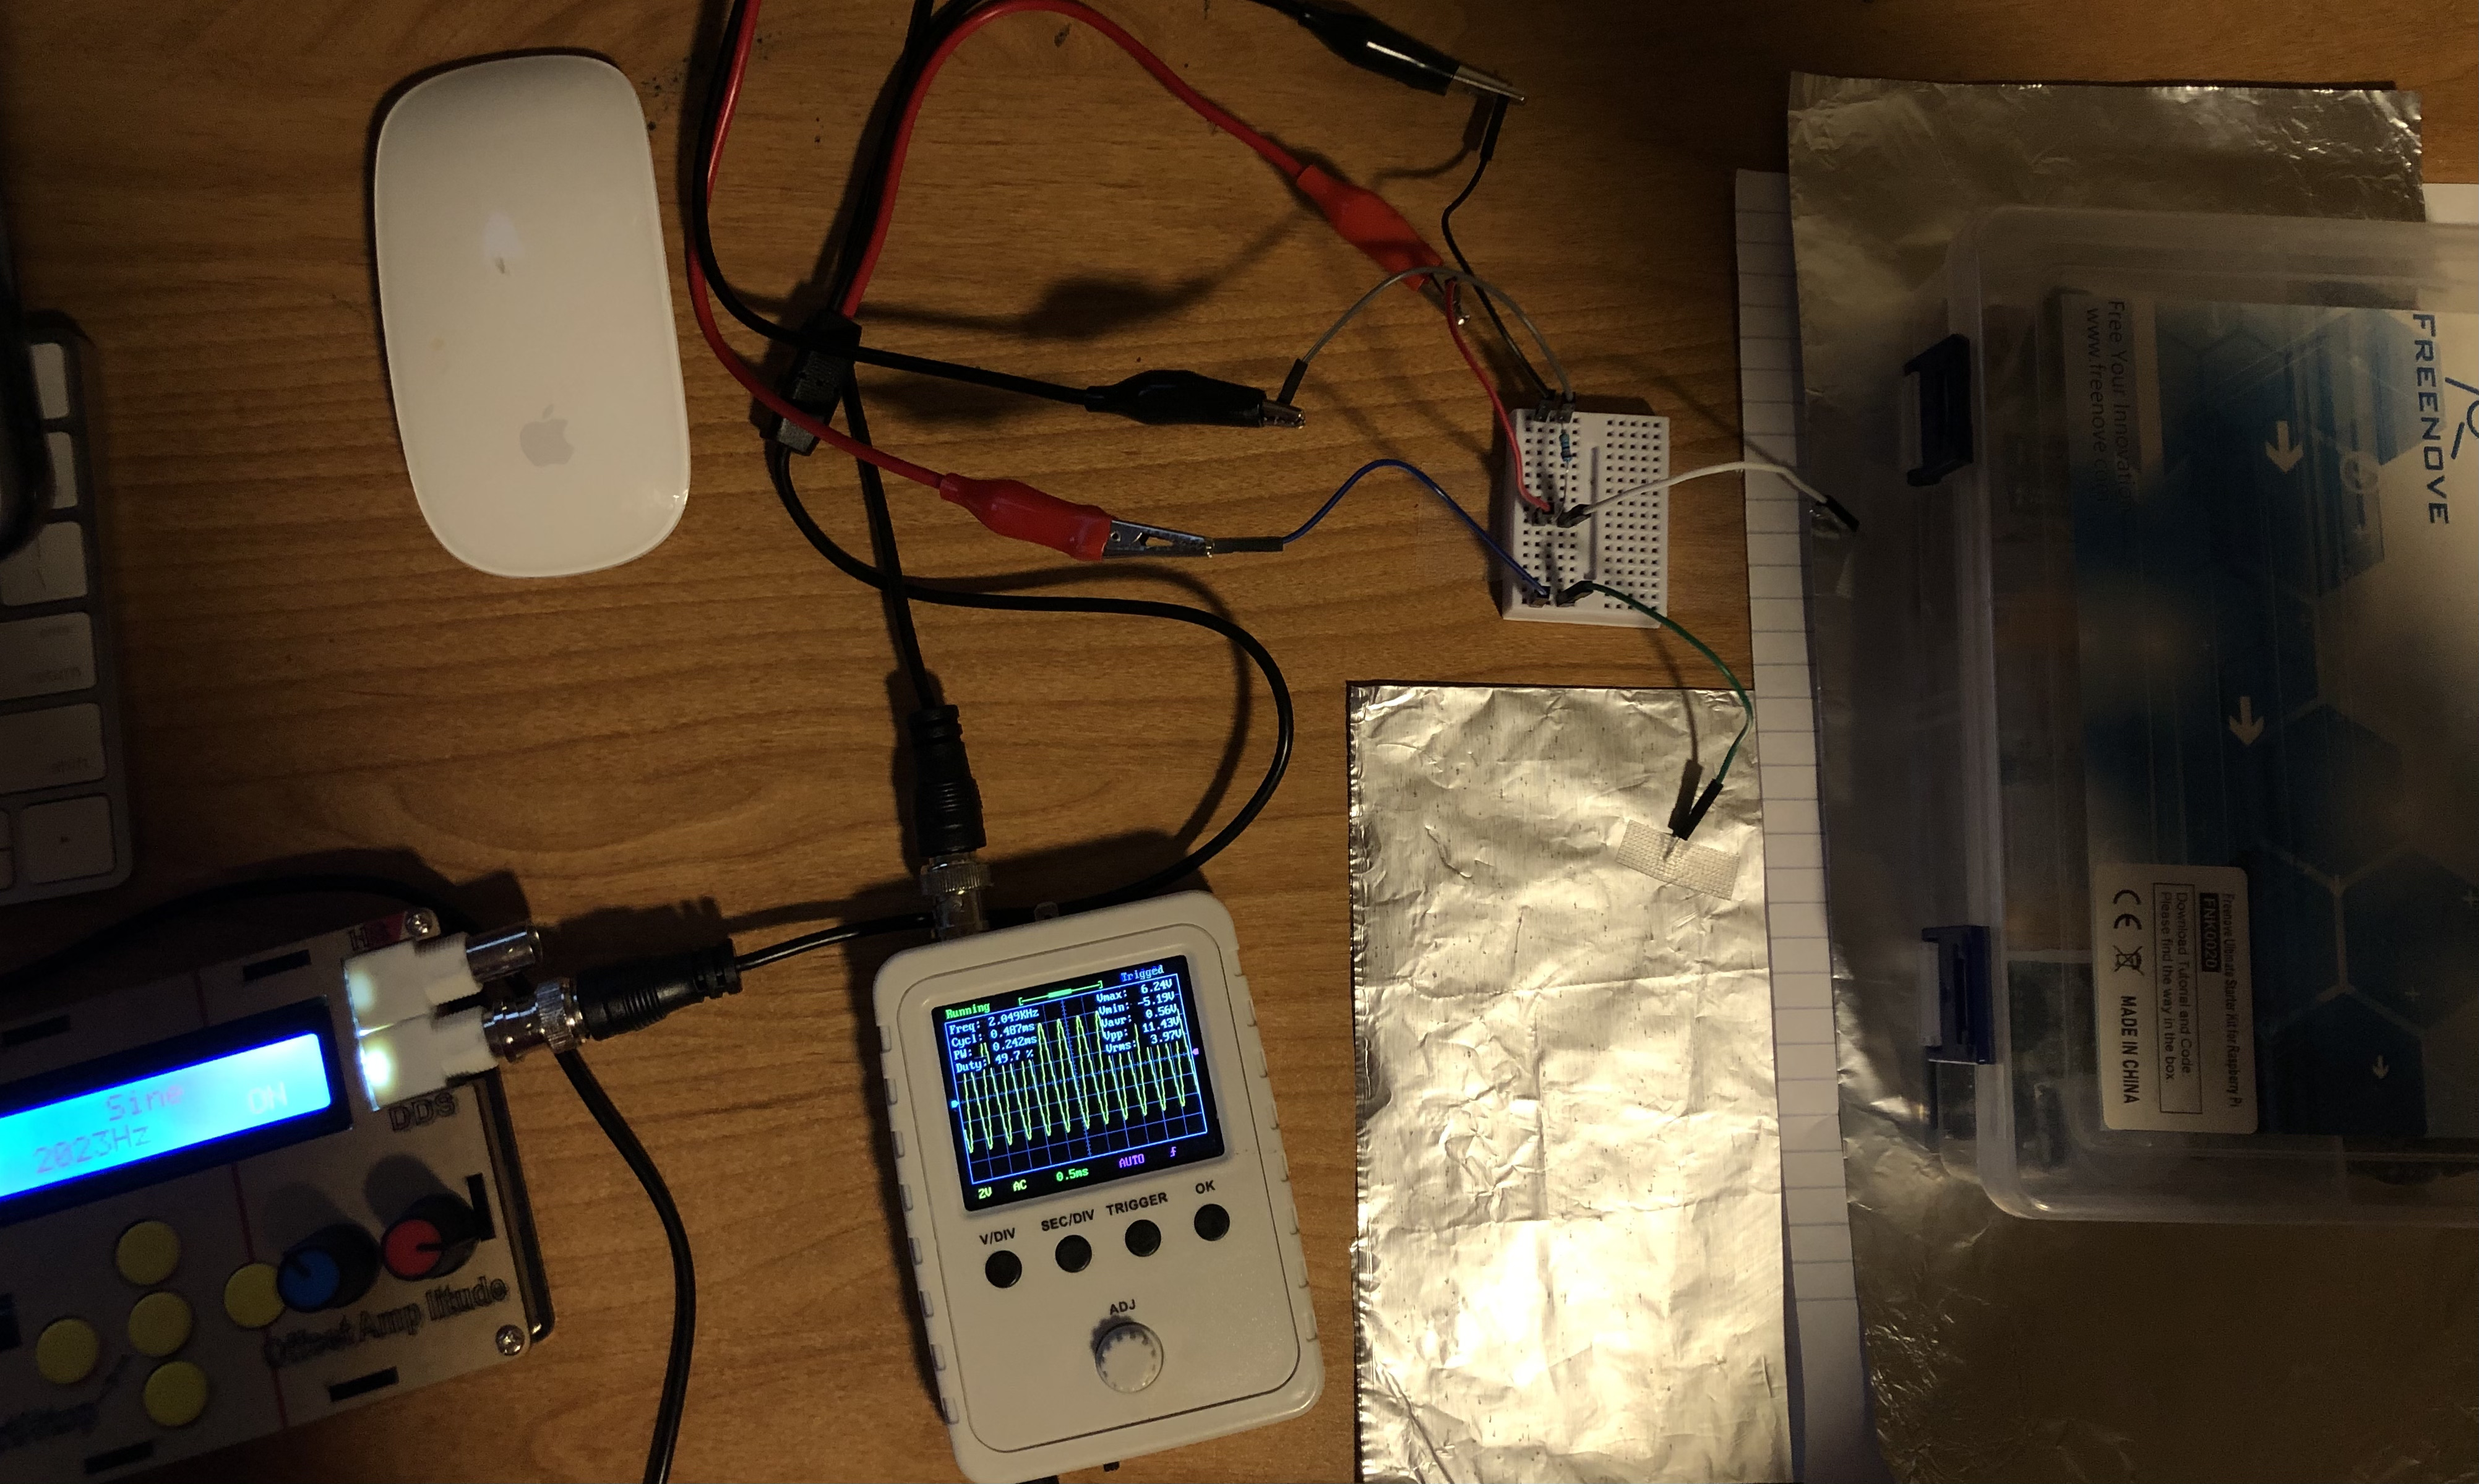
\includegraphics[scale=0.07]{VR.jpeg}
\end{center}

% \begin{center}
%   \subsection*{Graph 1}
%   % 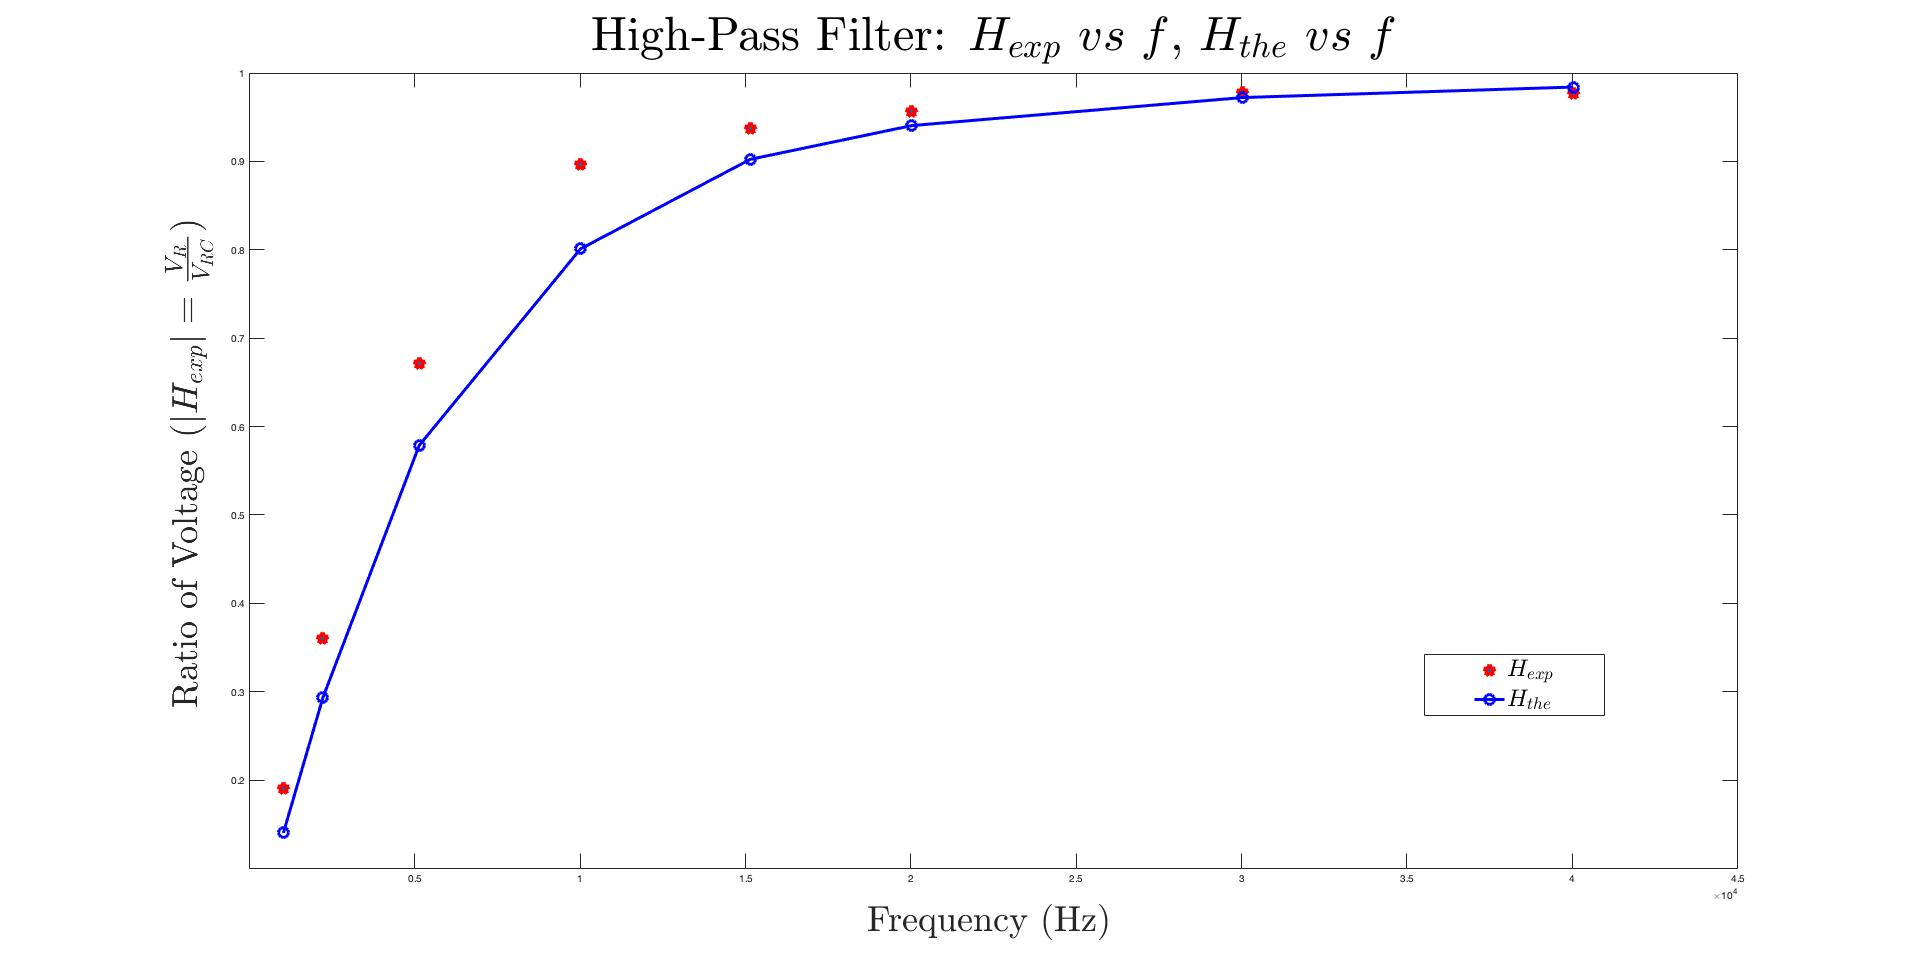
\includegraphics[scale=0.2]{graph1.jpg}
%   \subsection*{Graph 2}
%   % 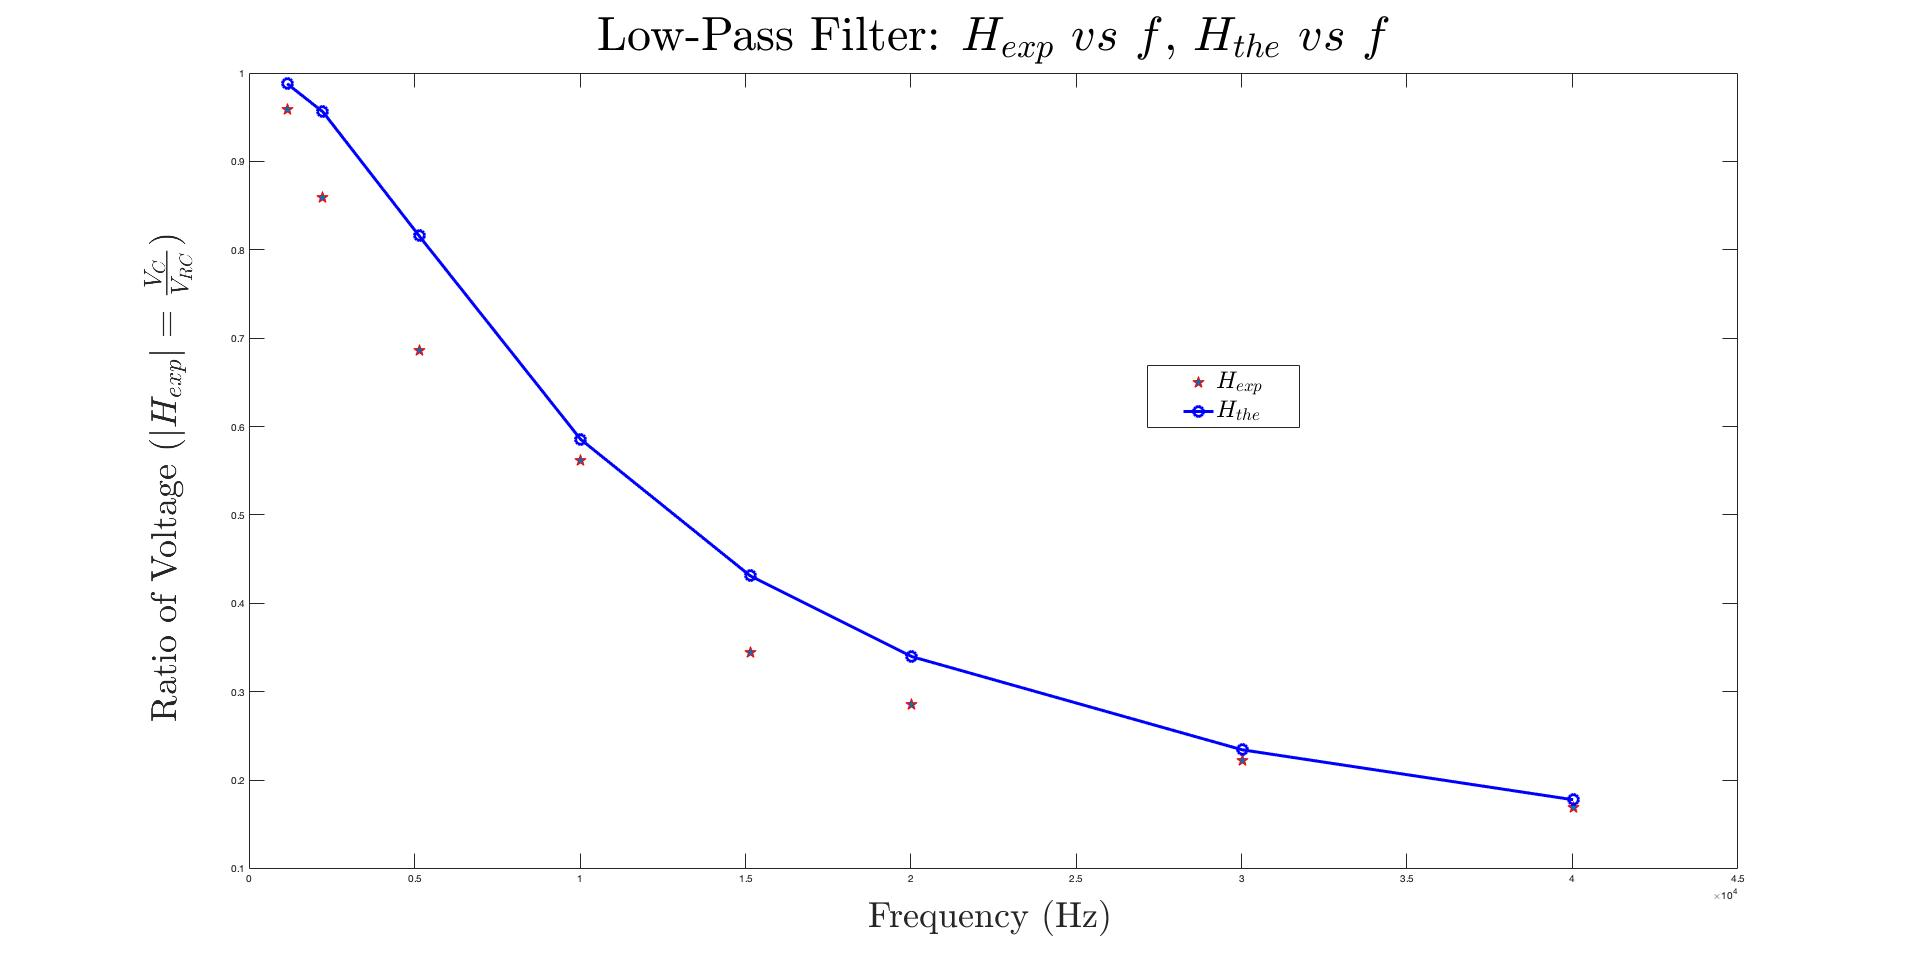
\includegraphics[scale=0.2]{graph2.jpg}
% \end{center}

\newpage
\begin{center}
  \begin{enumerate}
    \item Compare the theoretically obtained curves with the experimentally determined curves and quantify any difference. What do you think this difference is due to?
    \begin{itemize}
      \item
    \end{itemize}
  \end{enumerate}
\end{center}
\end{document}
